\section{Síťový analyzátor Wireshark}\label{wireshark}
Wireshark je grafická aplikace sloužící k zachytávání paketů a jejich analýze, viz obrázek \ref{fig:wireshark-layout}. Wireshark umí zachytávat provoz na lokálních fyzických či virtuálních síťových rozhraních počítače nebo zpracovávat zachycené pakety uložené v souboru typu PCAP. V případě zpracování příliš velkých souborů (stovky MB data) je vhodnější využívat pro zpracování řádkovou verzi nástroje Wireshark, která se nazývá {\tt tshark}\footnote{Viz \url{https://www.wireshark.org/docs/man-pages/tshark.html}}. Další populární nástroj pro odchytávání paketů a jejich zpracování je unixová aplikace \texttt{tcpdump}. 

\begin{figure}[h]
  \centering
  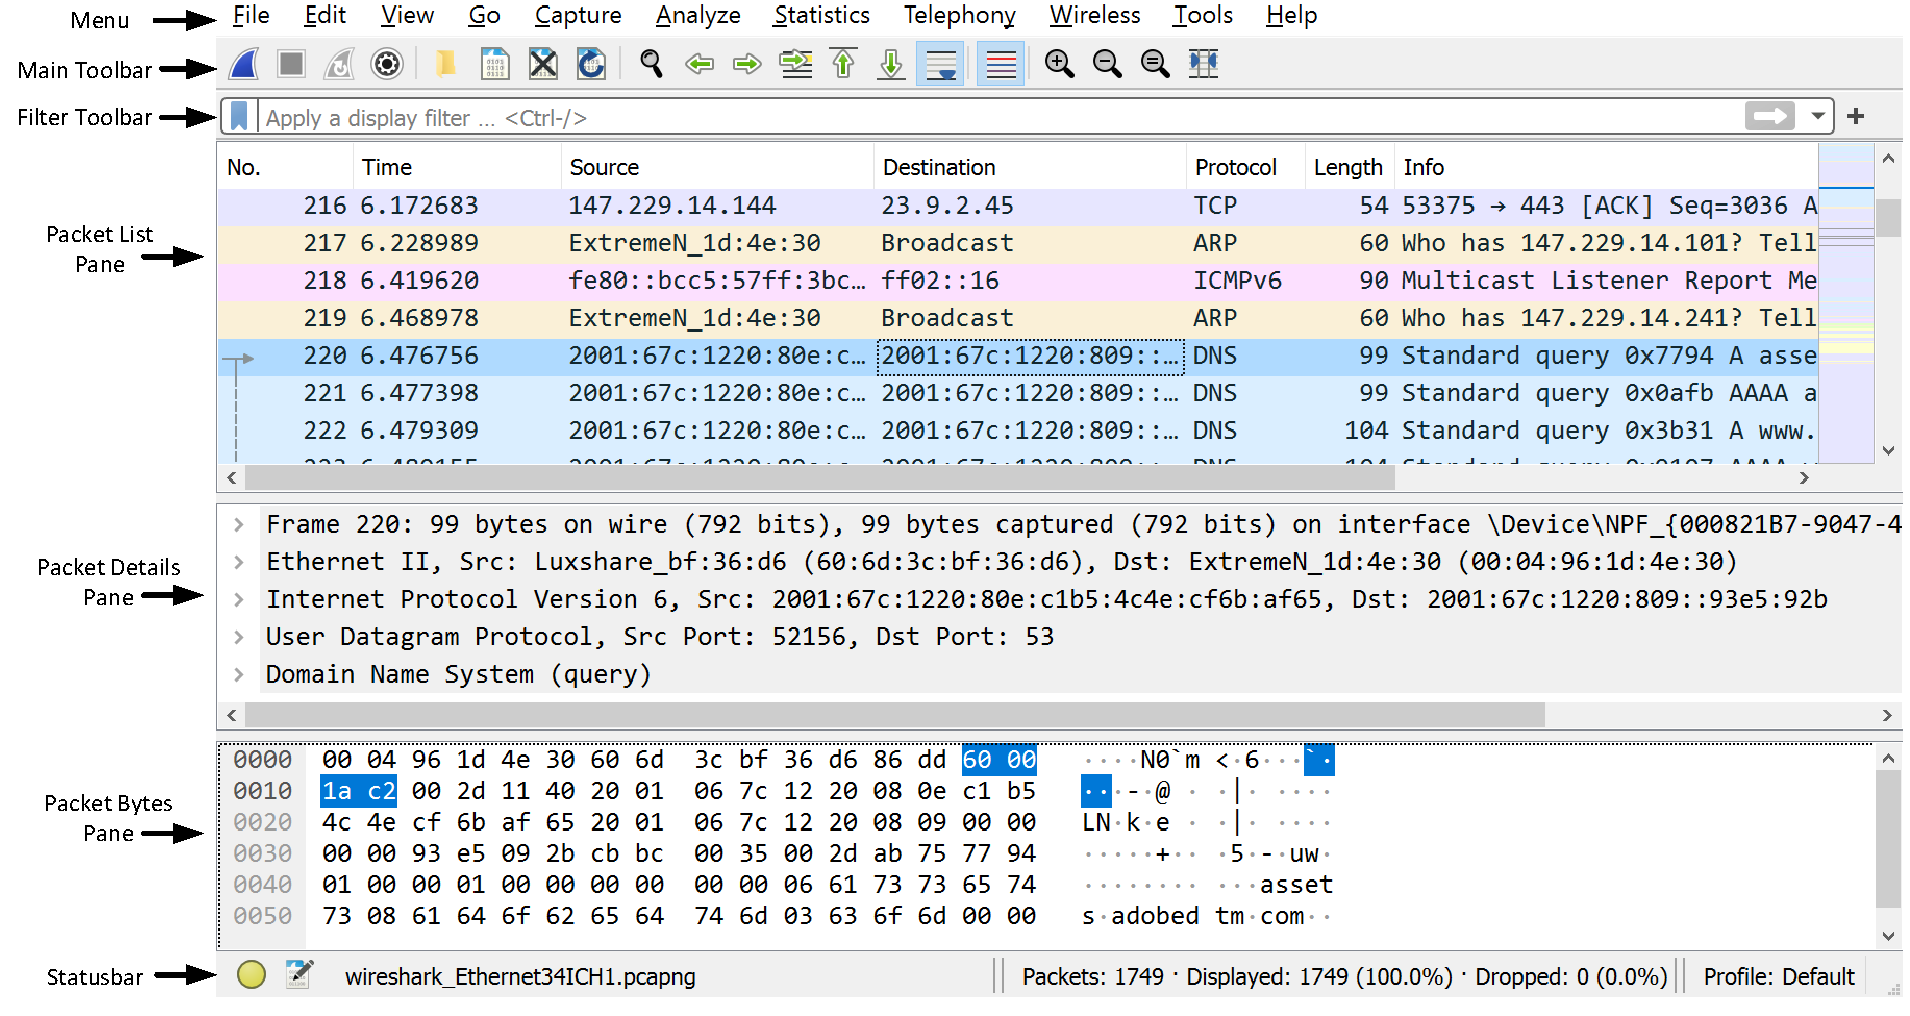
\includegraphics[width=170mm]{fig/wireshark-layout.pdf}
  \caption{Wireshark}\label{fig:wireshark-layout}
\end{figure}

\subsection{Zachytávání provozu (Packet Capturing)}
Následující kroky popisují proces zachytávání paketů v programu Wireshark:
\begin{enumerate}
  \item Zachytávat provoz můžeme z vybraného síťového rozhraní nebo z~více rozhraní najednou. Rozhraní vybereme v menu \texttt{Capture -> Options}.
  \item V nastavení Wiresharku je možné nastavit filtr pro výběr zachytávaných paketů (Capture Filter), pomocí kterého řekneme aplikaci, jaké pakety má zachytávat. Protože zpracování každého paketu je výpočetně náročné (dochází k parserování jednotlivých vrstev paketu a detekci protokolů), snížeme použití vstupního filtru výpočetní nároky na odchyt paketů. Políčko {\tt Capture Filter} umožňuje vybrat již předdefinovaný filtr nebo je zadat vlastní filtr, viz {\tt man pcap-filter}.
  \item Záchyt spustíme pomocí tlačítka \texttt{Start}.
  \item Odchycený provoz (tj. jednotlivé pakety spolu s časovými značkami) můžeme také uložit do souboru typu PCAP pro pozdější analýzu.
\end{enumerate}

\subsection{Výběr zachyceného provozu pomocí zobrazovacího filtru (Display Filter)}
Zachycené a zpracované pakety jsou zobrazeny v okně {\tt Packet List Pane}. Protože nás často zajímá pouze určitý provoz, např. komunikace HTTP s konkrétní stanicí, je vhodné využít zobrazovací filtr (Display Filter), který se nachází pod nástrojovou lištou. Pomocí tohoto filtru vybereme pouze pakety s požadovanou vlastností, např. filtr {\tt ip.addr == 147.229.8.12} vybere veškeré pakety, které mají danou zdrojovou či cílovou IP adresu. 

Základní operace pro vytváření zobrazovacího filteru je popsána v tabulce \ref{tab:display-filter}. 
\begin{center}
  \begin{table}[h]
    \centering
    \def\arraystretch{1.2}
    \begin{tabular}{|l|l|}
      \hline
      \textbf{Porovnávání} & \texttt{==, >=, <=, !=, contains}\\
      \textbf{Logické operátory} & \texttt{||, or, \&\&, and, !, not}\\
      \textbf{Kombinace filtrů} & \texttt{(ip.src==192.168.0.105 and udp.port==53)}\\
      \textbf{Filtrování na základě existence pole} & \texttt{http.cookie or http.set\_cookie}\\
      \textbf{Filtrování specifických bytů} & \texttt{eth.src[4:2]==22:1b}\\
      \textbf{Regex filtrování} & \texttt{http.host \&\& !http.host matches ".com"}\\
      \hline
    \end{tabular}
    \caption{Syntax zobrazovacího filtru (Display Filter)}\label{tab:display-filter}
  \end{table}
\end{center}

\subsection{Zobrazení toků (Flow Graph)}
Wireshark umožňuje zobrazit časovou posloupnost komunikace pomocí tzv. grafu toků zvaného \texttt{flow graph}, viz menu \texttt{Statistics -> Flow Graph}. Graf toků zobrazuje komunikaci mezi jednotlivými zařízeními definovanými IP adresou, viz obrázek \ref{fig:flow-graph}. Pomocí grafu toků můžeme vidět, jak často spolu stanice komunikují, jaké zprávy a v jakém pořadí si posílají a další.

\begin{figure}[h]
  \centering
  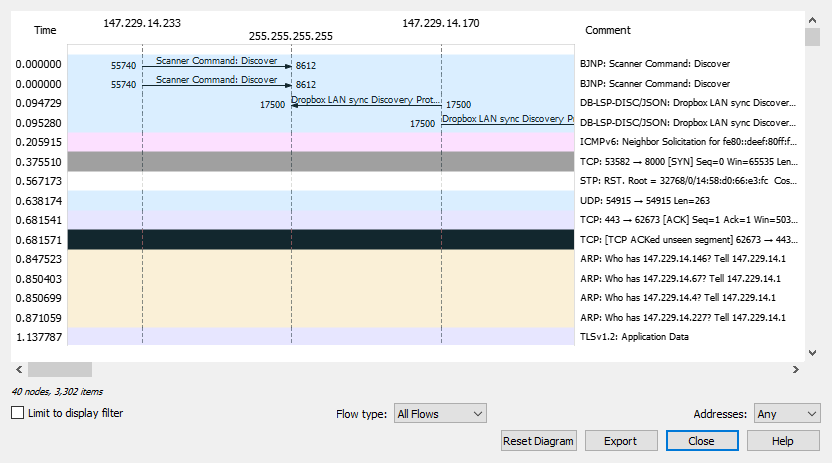
\includegraphics[width=110mm]{fig/flow-graph.png}
  \caption{Flow Graph}\label{fig:flow-graph}
\end{figure}

\subsection{Zobrazení obsahu toku (Stream Analysis)}
Wireshark zachytává jednotlivé pakety. Pokud chceme sledovat průběh celé komunikace včetně obsahu, můžeme  zobrazit danou komunikaci (streamu) pomocí volby \texttt{Flow <protokol> Stream}, např. TCP či UDP spojení, HTTP spojení apod. Zobrazení toku provedeme tak, že vybereme jeden zachycený paket daného toku, klikneme na něj pravým tlačítkem myši a vybereme volbu  \texttt{Follow <protokol> Stream}. Příklad obsahu HTTP komunikace je na obrázku \ref{fig:follow_stream}.

\begin{figure}[h]
  \centering
  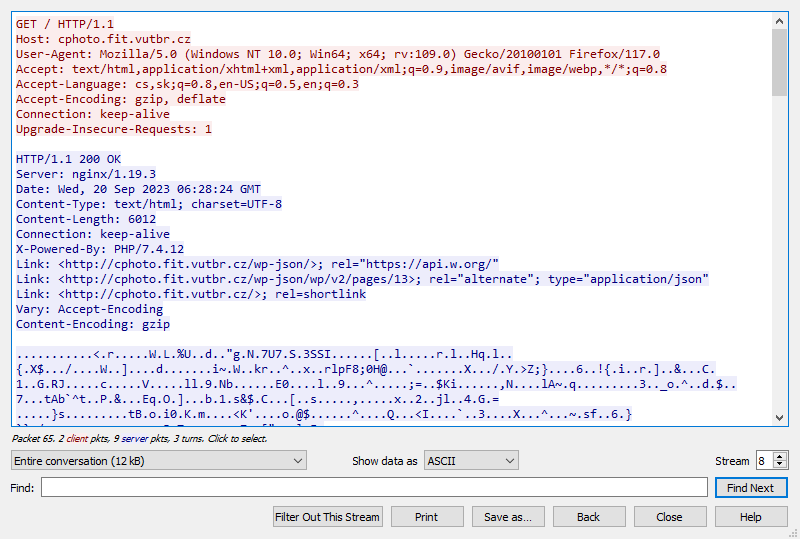
\includegraphics[width=110mm]{fig/follow_stream.png}
  \caption{Zobrazení toku HTTP}\label{fig:follow_stream}
\end{figure}

\subsection{Časové značky}
Každý paket obsahuje časovou značku svého záchytu. Zobrazení časové značky závisí na nastavení Wiresharku. Wireshark umožňuje zobrazit čas jako časovou značku obsahující datum a čas záchytu, absolutní čas, relativní čas od začátku záchytu komunikace a další. Formát času můžeme nastavit v menu \texttt{View -> Time Display Format}, viz obrázek \ref{fig:time-stamps}. Pro některé účely je vhodnější vidět pouze relativní čas od začátku záchytu paketů, pro jiné je potřeba znát absolutní čas záchytu. 

\begin{figure}[h]
  \centering
  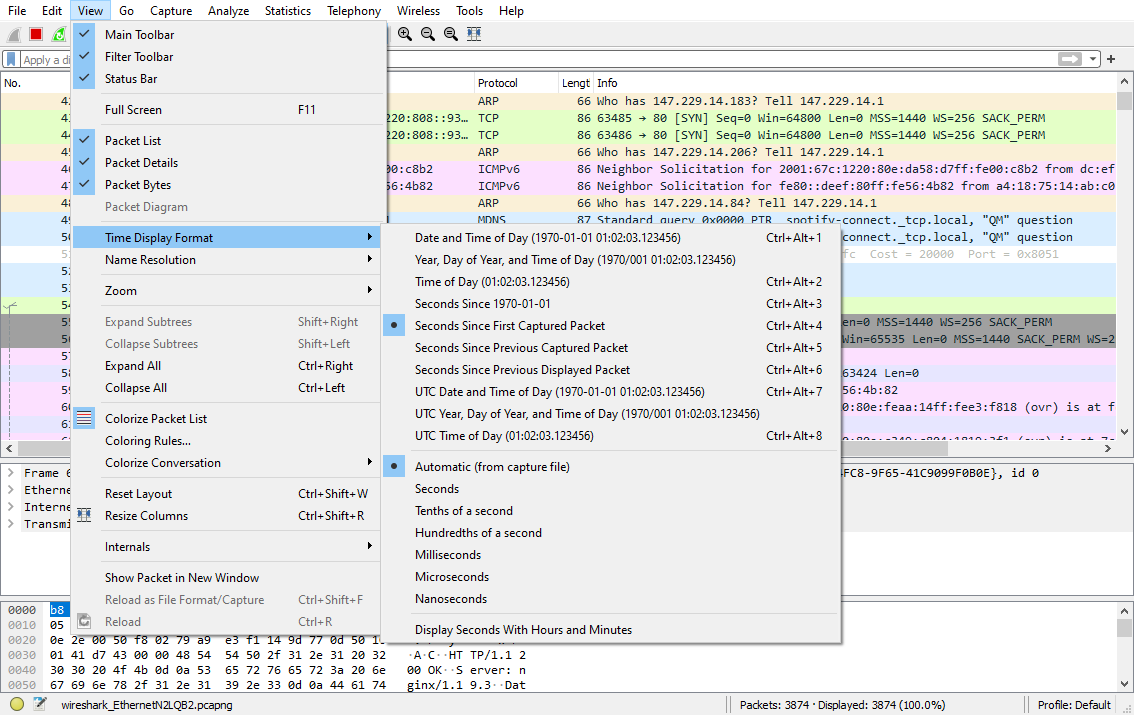
\includegraphics[width=110mm]{fig/time-stamps.png}
  \caption{Nastavení formátu časových značek}\label{fig:time-stamps}
\end{figure}
